% SSAC27 research paper competition abstract. Rules: fewer than 500 words including the
% title; sections Introduction, Methods, Results, Conclusion; at most two exhibits; a public
% repository link. No official class file is specified, so this uses article.
%
% Every number in Results is printed by make_comparison_figure.py (which reads evidence/*.json)
% or comes from the paper's own tables. The comparison uses the 1,892 validation player-games
% that all four evaluations score (see match_mdn_games.py). The shot-chart numbers are the
% corrected 2026-06-12 evaluation, NOT the reference column printed in paper/shot_cloud.tex:
% that older run passed player and game ids glued together, so every player fell back to the
% position-group density. The paper's claim that the autonomous rollout beats the reference
% does not survive the correction and is not made here.
\documentclass[11pt,letterpaper]{article}
\usepackage[margin=1in]{geometry}
\usepackage[T1]{fontenc}
\usepackage{lmodern,microtype,graphicx,booktabs,float}
\usepackage[font=small,skip=4pt]{caption}
\usepackage[hidelinks]{hyperref}
\setlength{\parindent}{0pt}
\setlength{\parskip}{3pt}
\pagestyle{empty}
\newcommand{\abstractsection}[1]{\par\vspace{3pt}\noindent\textbf{#1}\par\nobreak}
\author{Aaron John Danielson\\
The University of Texas at Austin\\
\href{mailto:aaron.danielson@austin.utexas.edu}{aaron.danielson@austin.utexas.edu}}
\hypersetup{pdftitle={Shot Clouds: Predicting Where an NBA Player Shoots in a Game},pdfauthor={Aaron John Danielson}}

\begin{document}
\begin{center}
{\large\bfseries Shot Clouds: Predicting Where an NBA Player Shoots in a Game}
\par\vspace{5pt}
{\small\makeatletter\@author\makeatother}
\end{center}
\vspace{-8pt}

\abstractsection{Introduction}
Scouting and lineup simulations need to know where a player will shoot in a game. The season shot chart [1] averages hundreds of attempts, while one game holds ten to thirty, so a single-game forecast is a distribution over small sets of shots, a \emph{shot cloud}. For rookies and players in new roles, own history is thin, so the forecast must borrow from similar players. We ask whether learning which individual past attempts matter for a given game yields more realistic shot clouds.

\abstractsection{Methods}
Using public NBA shot data (2014--2024), we train through June 2023 and evaluate on 2023--24. Each player-game is a marked point process of shot count, times and locations. Our central contribution is shot-level attention. Adaptive Collaborative KDE (AC-KDE) uses context-dependent attention to weight past shots from the player and from similar players, forming the predicted location density. A gate increases the weight on the player's own shots as his history grows, and the weights reveal which past attempts shape each forecast (Figure~\ref{fig:attention}). Predictions are conditional: they take the player's observed minutes and shot count and, at each attempt, the game clock and his earlier observed shots that game; all other inputs are known before tipoff. We score simulated clouds on six distances against a noise floor from resampling the observed cloud.

\abstractsection{Results}
On the 1,892 high-volume player-games every method scores (mean 22 shots), AC-KDE produces the most realistic clouds on all six measures, ahead of a position-only chart, the player's own shot chart and a mixture density network (every paired 95\% interval excludes zero; Figure~\ref{fig:comparison}). Mean shot-distance error is 3.00 feet for the position chart, 2.65 for the player's chart and 2.49 for AC-KDE. The network has lower per-shot negative log-likelihood (6.06 versus 6.15 nats) yet produces less realistic clouds: likelihood alone would have picked the wrong model. Replacing learned attention with equal weights on the same shots worsens all six measures (shot-distance error 2.49 to 2.58 feet). The weight on a player's own shots rises from 0.64 (under 92 prior attempts) to 0.92 (over 423).

\abstractsection{Conclusion}
The model learns which real shots to remember and how much weight to give each. Shot clouds give teams simulation-ready predictions for players with varying amounts of history, judged one game at a time.

\vspace{2pt}
{\small
\textbf{References}\par
[1] Goldsberry, K.\ (2012). CourtVision. \emph{MIT Sloan Sports Analytics Conference}.\par
Code: \url{https://github.com/aaronjdanielson/shot-cloud-generation}
}

\clearpage
\begin{figure}[H]
\centering
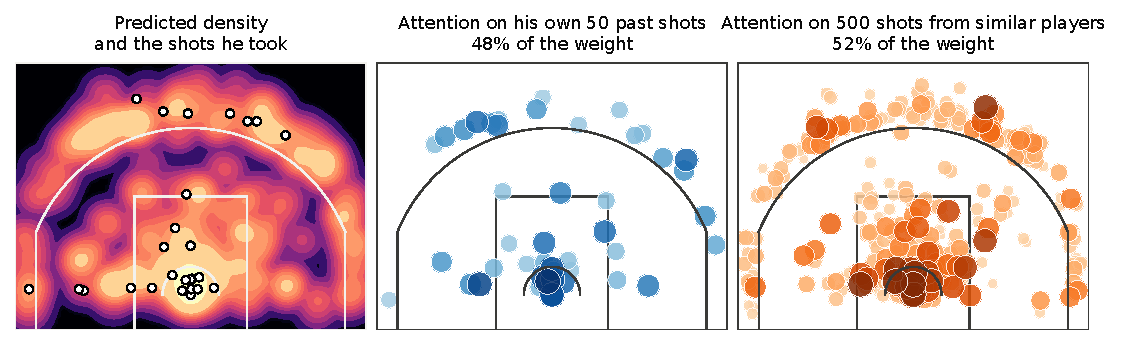
\includegraphics[width=\linewidth]{figures/fig_attention.pdf}
\caption{AC-KDE forecast for one rookie game (Victor Wembanyama, 26 shots). Left: predicted density, observed shots in white. Middle and right: each dot is a past shot; larger, darker dots carry more attention.}
\label{fig:attention}
\end{figure}

\begin{figure}[H]
\centering
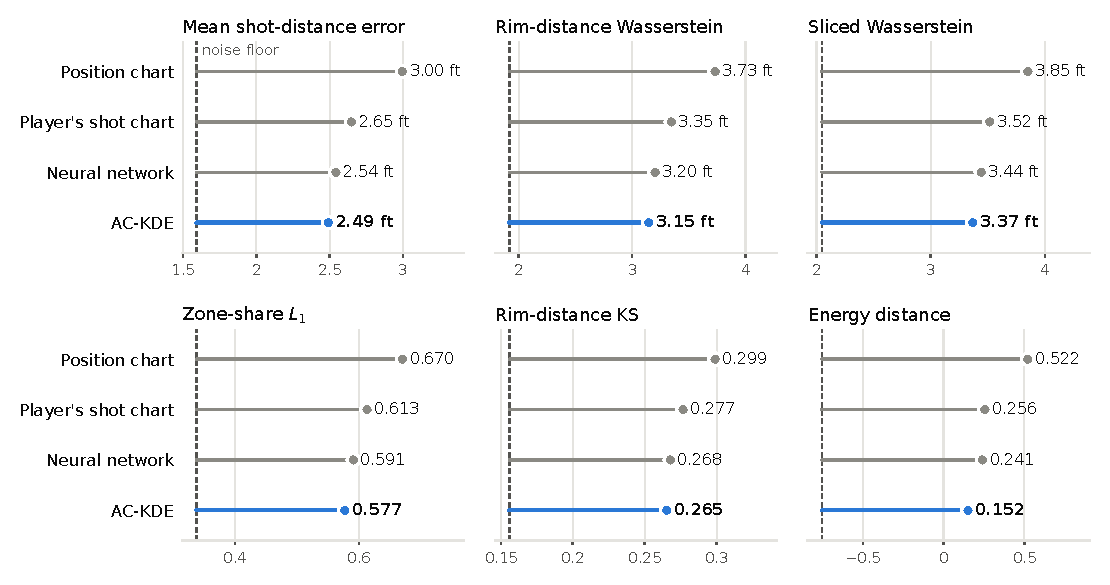
\includegraphics[width=\linewidth]{figures/fig_method_comparison.pdf}
\caption{Shot-cloud error on the same 1,892 player-games from 2023--24 (lower is better; dashes: noise floor). Position chart: his position group's shot density.}
\label{fig:comparison}
\end{figure}
\end{document}
